\documentclass[10pt]{article}
\usepackage{icmlko}

\icmlmeta{IP 파운데이션 월드모델}{21}{순위는 공짜, 눈금은 여덟 건}{절대량을 얻는 데 필요한 대상 라벨 수를 쟀다 --- 아이돌은 여덟 건에서 상수를 90\% 이긴다}

\begin{document}

\twocolumn[
\icmlheader

\begin{abstract}
노트 19의 파이프라인은 라벨 0개로 예측하지만 도메인 내 표준화 눈금에서만 그렇다.
실무에는 숫자가 필요하다 --- ``상위 30\%''가 아니라 ``하루 1,200명''이어야 기획이
선다. 이 노트는 순위와 눈금의 비용을 분리해 잰다. \textbf{순위는 라벨 0개고,
눈금은 중심과 폭 두 모수뿐이므로 소수의 라벨로 추정된다.} 결과를 배수 오차로
낸다 --- 평균 몇 배 틀리는가. \textbf{아이돌에서 여덟 건이면 상수를 90\% 이긴다}
(4.28배 대 4.86배). 스무 건이면 3.96배 대 4.64배로 벌어진다. 팝업은 열두 건부터
근소하게 앞선다(2.79배 대 2.82배, 승률 65\%). \textbf{게임에서는 쓰면 안 된다} ---
전 구간에서 지고 k가 커질수록 나빠진다(k=50에서 승률 0.04). 이는 노트 13부터
반복된 패턴 --- 게임은 좋은 출처이고 나쁜 대상이다 --- 이 절대량 단계에서도
유지된다는 뜻이다. 부수적으로 방법 하나를 고쳤다. 폭 추정에 표준편차 대신
중앙절대편차를 쓰면 \emph{참 분포의 표준편차를 아는 경우보다도} 낫다
(아이돌 3.96배 대 4.31배) --- 평균절대오차를 최소화할 때는 로버스트 추정이
맞는 눈금이다.
\end{abstract}
]

\section{순위와 눈금은 다른 비용이다}

노트 19가 라벨 0개 파이프라인을 완성하며 남긴 한계는 이랬다.

\begin{quote}\fontsize{9.2}{11}\selectfont
이 파이프라인은 순위를 맞히지 절대량을 맞히지 못한다. 도메인 안에서 표준화한
눈금이므로, 실제 방문자 수를 얻으려면 그 도메인의 분포를 알아야 한다.
\end{quote}

분포를 알려면 라벨이 필요하다. 그런데 \emph{얼마나} 필요한지는 재보지 않았다.
여기서 두 가지가 분리된다.

\begin{figure}[t]
\centering

\includegraphics[width=\columnwidth]{figs/split.pdf}
\caption{두 부분의 비용이 다르다. 순위는 구조에서, 눈금은 표본에서 온다.}
\end{figure}

\begin{itemize}[leftmargin=1.1em,itemsep=0.15em]
\item \textbf{순위} --- 프로크루스테스 정렬과 전이 계수로 얻는다. 대상 라벨 0개
      (노트 19).
\item \textbf{눈금} --- 잔차 분포의 중심과 폭, 모수 둘. 라벨 몇 개면 추정된다.
\end{itemize}

시간 추세는 라벨이 필요 없다는 점도 중요하다. 관측 시점만 알면 계산되므로 k에
들어가지 않는다.

\paragraph{노트 16의 실험과 다르다}
거기서는 기울기와 절편을 자유롭게 맞춰 \emph{순위 자체}를 바꾸려 했고 실패했다
(k=2에서 팝업 MAE가 8.97까지 폭주). 여기서는 순위를 그대로 두고 눈금만 옮긴다.
자유도가 훨씬 적다.

\paragraph{배수 오차로 읽는다}
성적을 log10 공간의 평균절대오차로 내면 실무자가 읽을 수 없다. 10의 거듭제곱으로
되돌리면 ``평균 몇 배 틀리는가''가 된다. 2.8배는 1,000명 예측이 실제로는 360명에서
2,800명 사이라는 뜻이다.

\section{아이돌은 여덟 건이면 된다}

\begin{figure}[t]
\centering

\includegraphics[width=\textwidth]{figs/curve.pdf}
\caption{눈금에 쓴 라벨 수에 따른 배수 오차. 점선은 참 분포를 안다고 가정한
경우(중앙절대편차 기준).}
\end{figure}

\begin{table}[t]
\centering\tsize
\caption{아이돌(n=63). 배수 오차, 200회 반복.}
\begin{tabular}{rrrr}
\toprule
k & 파이프라인 & 상수 & 이긴 비율 \\
\midrule
3 & 5.62배 & 5.88배 & 84\% \\
5 & 4.85배 & 5.30배 & 85\% \\
\textbf{8} & \textbf{4.28배} & 4.86배 & \textbf{90\%} \\
12 & 4.15배 & 4.84배 & 90\% \\
20 & 3.96배 & 4.64배 & 89\% \\
30 & 3.85배 & 4.61배 & 86\% \\
\midrule
전량 & 3.65배 & --- & --- \\
\bottomrule
\end{tabular}
\end{table}

여덟 건에서 이미 승률 90\%다. 스무 건이면 3.96배 대 4.64배로 15\% 앞선다. 라벨을
전부 쓴 경우(3.65배)와의 거리도 스무 건에서 상당히 좁혀진다.

\claimx{순위를 라벨 없이 얻고 눈금만 소수 라벨로 잡는 방식이 작동한다. 아이돌
도메인에서 여덟 건이면 상수를 90\% 이기고, 스무 건이면 배수 오차가 15\% 줄어든다.}{새
도메인에서 여덟 건으로 승률이 절반을 못 넘으면, 이 결과는 아이돌 표본의
특성이었던 것이다.}

\section{팝업은 근소하고 게임은 진다}

\begin{figure}[t]
\centering
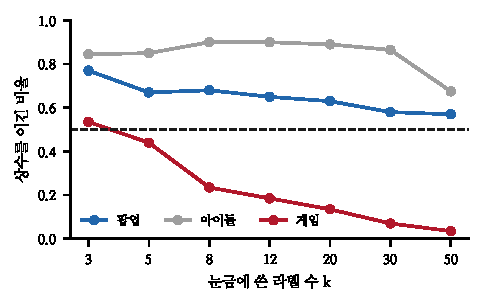
\includegraphics[width=\columnwidth]{figs/win.pdf}
\caption{도메인별 승률. 게임에서는 라벨을 더 줄수록 나빠진다.}
\end{figure}

\begin{table}[t]
\centering\tsize
\caption{팝업(n=75)과 게임(n=482). 배수 오차.}
\begin{tabular}{rrrrrrr}
\toprule
& \multicolumn{3}{c}{팝업} & \multicolumn{3}{c}{게임} \\
k & 파이프 & 상수 & 승률 & 파이프 & 상수 & 승률 \\
\midrule
5 & 3.17 & 3.02 & 67\% & 4.80 & 4.11 & 44\% \\
12 & 2.79 & 2.82 & 65\% & 4.57 & 3.81 & 18\% \\
30 & 2.69 & 2.70 & 58\% & 4.29 & 3.64 & 7\% \\
50 & 2.61 & 2.71 & 57\% & 4.24 & 3.59 & 4\% \\
\bottomrule
\end{tabular}
\end{table}

팝업은 열두 건부터 상수를 근소하게 앞선다. 승률이 0.57에서 0.68 사이로 아이돌만큼
분명하지 않다.

게임은 전 구간에서 진다. 그리고 \emph{라벨을 더 줄수록 나빠진다} --- k=5에서
승률 44\%였다가 k=50에서 4\%다. 눈금이 정확해질수록 잘못된 순위가 그대로
드러나기 때문이다.

이것은 노트 13부터 반복된 패턴의 연장이다 --- 게임은 좋은 출처이고 나쁜 대상이다.
순위 전이 단계에서 이미 그랬고(아이돌 $\to$ 게임 p=0.41), 절대량 단계에서도 같다.

\claimx{순위 전이가 실패하는 도메인에서는 절대량 복원도 실패하며, 라벨을 더 줄수록
악화된다. 눈금은 순위를 고쳐 주지 않는다.}{순위 전이가 유의하지 않은데 절대량
복원이 상수를 이기는 경우가 나오면, 두 단계가 독립이라는 뜻이다.}

실무 지침은 명확하다. \textbf{순위 전이의 유의성을 먼저 확인하고, 유의하지 않으면
절대량 단계로 넘어가지 않는다.}

\section{부수 발견 --- 폭 추정에는 중앙절대편차}

처음에는 참 분포를 아는 경우를 ``상한''으로 두었다. 그런데 k가 커지자 그 값을
넘어섰다 --- 아이돌 k=20에서 3.96배인데 ``상한''이 4.31배였다.

원인은 폭 추정 방법이었다. 참 분포 쪽은 표준편차를 썼고 k-표본 쪽은
중앙절대편차$\times$1.4826을 썼다. 평균절대오차를 최소화할 때는 로버스트
추정이 맞는 눈금이다.

\begin{table}[t]
\centering\tsize
\caption{참 분포를 알 때의 배수 오차, 폭 추정 방법별.}
\begin{tabular}{lrr}
\toprule
도메인 & 표준편차 & 중앙절대편차 \\
\midrule
아이돌 & 4.31배 & \textbf{3.65배} \\
게임 & 4.43배 & \textbf{4.04배} \\
\bottomrule
\end{tabular}
\end{table}

표기를 고쳤다. ``상한''이라 부르던 것은 상한이 아니었고, 중앙절대편차로 잡은
쪽이 실제 상한이다.

\claimx{예측을 평균절대오차로 평가하면 분포의 폭도 중앙절대편차로 잡아야 한다.
표준편차를 쓰면 참 분포를 알고도 소수 표본 추정에 진다.}{제곱오차로 평가하는
설정에서는 반대가 되어야 한다. 그렇지 않으면 이 규칙은 평가 지표와 무관한
것이다.}

\section{그래서 실무 절차}

\begin{enumerate}[leftmargin=1.3em,itemsep=0.2em]
\item 새 접점에서 축을 잰다(타깃 폭, 굿즈 규모). \textbf{라벨 0개.}
\item 인자 공간을 뽑아 기준 도메인에 회전 정렬한다. \textbf{라벨 0개.}
\item 순열 검정으로 전이가 유의한지 확인한다. 유의하지 않으면 여기서 멈춘다.
\item 유의하면 \textbf{8건에서 20건}을 실측해 잔차의 중심과 중앙절대편차를 잡는다.
\item 순위 예측에 그 눈금을 얹어 절대량을 낸다.
\end{enumerate}

배수 오차는 팝업 2.6에서 2.8배, 아이돌 3.9에서 4.3배다. 넓지만 상수보다 낫고,
무엇보다 \emph{새 도메인에서 8건만 실측하면 된다}는 점이 실무적으로 다르다.

\section{한계}

\begin{itemize}[leftmargin=1.1em,itemsep=0.15em]
\item 배수 오차 2.6에서 4.3배는 크다. 1,000명 예측이 실제로 380명에서 2,600명
      사이라는 뜻이다. 순위 판단에는 쓸 수 있어도 정산 근거로는 못 쓴다.
\item k개 라벨은 무작위 추출을 가정한다. 실무에서는 먼저 열리는 것부터 실측하므로
      시간 순서가 섞인다.
\item 게임의 실패가 순위 전이 실패에서 온다는 것은 논증이다. 순위를 인위적으로
      개선한 뒤 절대량이 따라 오르는지 확인해야 한다.
\item 팝업의 우위가 근소해 표본 재추출로 뒤집힐 수 있다.
\end{itemize}

\section{다음}

\begin{enumerate}[leftmargin=1.3em,itemsep=0.15em]
\item 미디어 투입을 도메인 독립 물리량으로 재정의 --- 노트 20이 남긴 과제.
\item 시간 순서를 지킨 k개 추출로 재검정 --- 실무 조건에 맞춘다.
\item 배수 오차를 줄이는 경로 탐색 --- 축을 늘리는 것과 표본을 늘리는 것 중 어느
      쪽이 효율적인지.
\item 네 번째 도메인에서 절차 전체를 그대로 적용.
\end{enumerate}

\vspace{0.6em}
\hrule height 0.3pt
\vspace{0.5em}
{\footnotesize
\textbf{참고문헌}\\[0.3em]
Rousseeuw, P. J., Croux, C. (1993). Alternatives to the median absolute deviation.
\emph{JASA}, 88(424), 1273--1283.\\[0.15em]
Huber, P. J. (1981). \emph{Robust Statistics}. Wiley.\\[0.15em]
Schönemann, P. H. (1966). A generalized solution of the orthogonal Procrustes
problem. \emph{Psychometrika}, 31(1), 1--10.\\[0.15em]
Ben-David, S. et al. (2010). A theory of learning from different domains.
\emph{Machine Learning}, 79(1--2), 151--175.
}

\end{document}
